\chapter{ICT investment and Wage Shares}

% \cite{Acemoglu2003}

% \cite{Adermon2011} - Sweden.



Since the late 1990s, both in Europe and the United States, the data show a marked polarization in the work force \citep{Goos2007, Autor2006}. This polarization has simultaneously manifested in \emph{wages} and in \emph{jobs}: both wage growth and growth in the level of employment are concentrated in high-skill jobs, and to a lesser extent, the bottom end of the skill spectrum. Middle-skill jobs have stagnated since the 1990s, both in terms of remuneration and level. The recent rise of ICT investment by firms has been attributed for this trend, both because many middle-skilled jobs can be substituted by computer capital, and because communications technologies enable firms to out source non-customer-facing roles to remote locations in order to take advantage of cheaper labor.

Computers, despite their sophistication, are only capable of performing a very limited set of simple, routine tasks. They excel at processes which require calculation and simple symbolic manipulation, and are not prone to the same types of errors as human workers. It is this fact which has led to their widespread adoption in automated tellers and a wide range of electronic service delivery which were formerly the domain of human personnel. Yet, any task that requires abstract thought or physical coordination, however elementary it may appear to a human worker, is not yet possible with a machine. Under this definition, many occupations which we might colloquially consider `routine'---such as stacking shelves or driving a taxi---require a degree of perception and motor control out of reach for a computer, and for our purposes are `non-routine.' In these areas, for the moment at least, human workers enjoy a competitive advantage, and technology is not yet a substitute \citep{Levy2003}.

Thus computing capital is a complement to some kinds of task-performing labor, and a substitute for others. As \citet{Levy2003} show, in the United States between 1960 and 1998, computerization led to a substitution in the observed levels of employment, away from routine tasks and toward cognitive tasks. Non-routine tasks, on the other hand, may improve, rather than replace, the efficiency of human workers. Indeed, as \citet{Borland2004} found by studying the computer knowledge of a cross-section of Australian workers surveyed in 1992, computer knowledge accrues a skill premium of around 10\%. Likewise, \citet{Goos2007} show a similar trend in the United Kingdom: between 1975 and 2003, they find an increase in the number of ``lovely'' (high-skill, high-wage) jobs and ``lousy'' (low-wage, low-skill) jobs, but a relative decrease in the number of ``middling'' jobs. In a subsequent paper, a similar pattern was found for most of Continental Europe \citep{Goos2009}.

The task approach departs from the standard neoclassical production function, which views aggregate economic output as a simple function of inputs such as capital and labor, but does not consider the specifics of the processes which produced that output \citep{Acemoglu2011}. Although the canonical approach has been very successful in explaining aggregate output levels, it is not sensitive to qualitative changes in the nature of production such as changes in the technology which produce output. 

\section{Model}

To test this pattern for Australian data, we can augment \eqref{eq:prod} by introducing a third type of labor, $M$, to represent work which requires mid-level skill and low levels of physical activity, representing `routine' or `middling' work. We also introduce computer capital, $C$, as a substitute in production for medium-skilled labor, and a complement in production for high-skilled workers:
\begin{equation}  \label{eq:prod2}
Y = \left[
  \left(A_LL \right)^\frac{\sigma-1}{\sigma}
  +
  \left(A_MM + C\right)^\frac{\sigma-1}{\sigma}
  +
  \left((A_HH)^\mu + C^\mu\right)^\frac{\sigma-1}{\mu\sigma}
  \right]^\frac{1}{\sigma-1}.
\end{equation}
\citet{Michaels2010} use a formulation similar to \eqref{eq:prod2} to show that, if ICT investment $C$ increases exogenously, the wage share for high-skill workers should increase, but decrease for low-skill workers. Likewise, the wage premium for high-skilled workers should rise with increasing ICT investment, and fall for medium-skilled workers.\footnote{Following \citet{Michaels2010}, we focus on the wage {\em share}, and not the absolute wage. Although wages for high-skilled and low-skilled workers should increase with increased investment, the comparative static predictions for medium-skilled workers are indeterminate. Michaels et al. prove that the comparative static predictions for the wage share, however, are unambiguous.} To test these predictions, \citet{Michaels2010} specify a simple translog flexible functional form to test the impact of ICT investment on the wage share for type of labor $S\in\{H,M,L\}$, estimated for broad industry groups across eleven countries, using educational attainment as a proxy for skill. The authors find support for the claim that ICT investment is associated with a decrease in the demand for middle-skilled labor. 

Adapting their specification for Australia gives the empirical model shown below. In this model, $SHARE^S$, computed as ${\sum_k W^S_k/\sum_{s,j}W^s_j}$ is the wage bill share for the labor category $S$, $C$ is ICT capital, $K$ is non-ICT capital, and $Q_i$ is value added by industry $i$. 
\begin{equation} \label{eq:translog}
\Delta SHARE^S = \alpha_{CS}\log(C/Q)_{it} + \alpha_{KS}\log(K/Q)_{it} + \alpha_{QS}\log(Q)_{it}.
\end{equation}
As Michaels {\it et al.} point out, the polarization hypothesis is consistent with $\alpha_{MS}<0$ and $\alpha_{HS}>0$.

With the results from the previous section in mind, to adapt this specification for Australia requires an alternative yard-stick for `skill.' Following \citet{Levy2003}, we partition occupations according to the tasks they involve, according to the occupational classification coded in the SIH. For the purposes of this very simple and informal model, we divide occupations into three categories: `non-routine manual' (low-skilled), `routine' (middle-skilled), and `non-routine cognitive' (high-skilled.) Capital series were derived from national accounting data. Our data include two different measures of ICT capital: {\em software}, and {\em electrical and electronic equipment}. Software includes both commercial off-the-shelf packages, as well as custom-built line-of-business programs, whereas the second variable includes telecommunications equipment and other electronic machinery. To smooth out variation in the data, the  period 1996-2010 was divided into two seven-year periods.

\subsection{Results}

The results from estimating \eqref{eq:prod2}, given in Table~\ref{tbl:reg}, lend mixed support for the polarization hypothesis. While estimates for $\alpha_{MS}<0$ and $\alpha_{HS}>0$ have the expected sign, they are not significant when estimated with all the parameters specified in $\eqref{eq:translog}$. However, with just electrical and electronic equipment included in regression, $\alpha_{MS}<0$ is negative and significant at the 5\% level. Column (4) of Table~\ref{tbl:reg} suggests that, over a seven-year period, a 10\% increase in electrical and electronic equipment capital is associated with a decrease in the wage share of middle-skilled workers of around 0.2, whereas it is associated with a relative increase in the wage share of high-skill workers versus low-skilled workers.

The sign of coefficient estimates for the {\em software} variable are opposites in all estimates. This suggests that software capital may in fact be a complement to medium-skilled labor. Since {\em equipment} includes telecommunications infrastructure, one interpretation is that {\em outsourcing}, rather than a direct application of labor-saving capital, is responsible for the decline in middle-skill labor.

\begin{figure}
  \centering
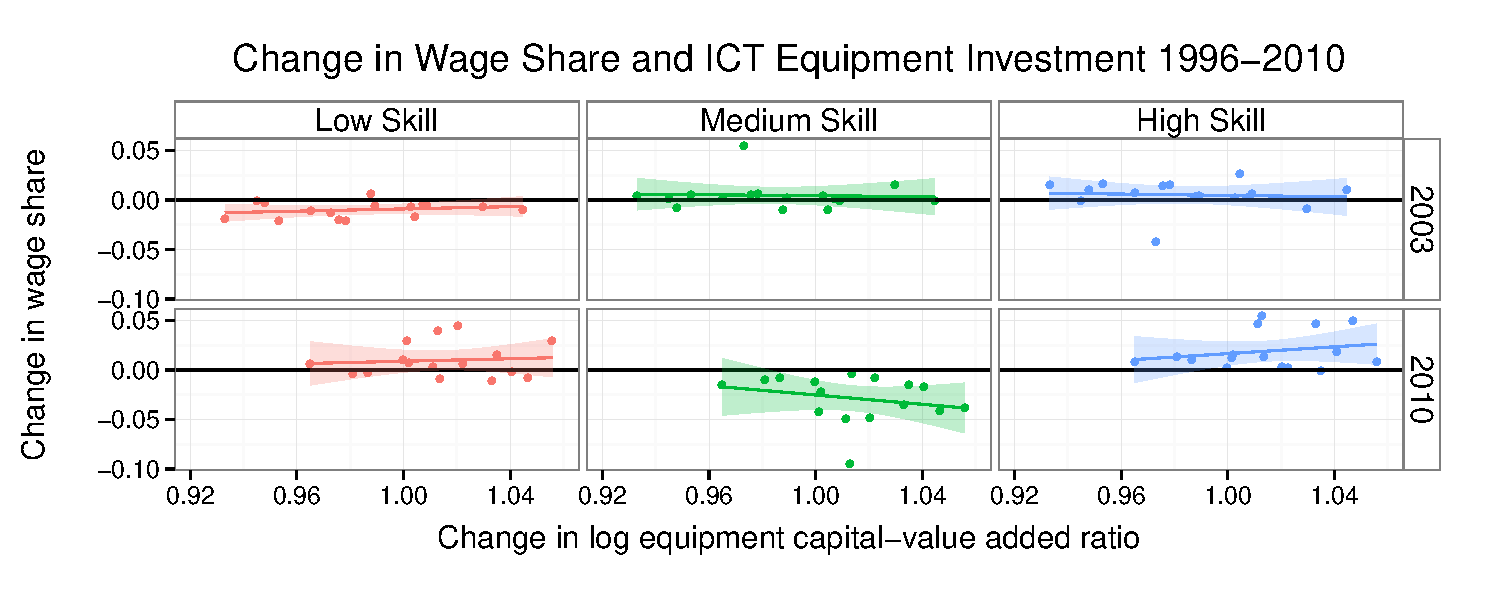
\includegraphics[width=0.8\textwidth]{../figure/wage_share_equipment_skill_split.pdf}
  \caption{Change in wage share against change in log ICT electrical and electronic equipment capital ratio, by industry, Australia, 1996-2010.
    Fitted line comuted using LOESS regression and 95\% confidence interval. See note for Table~\ref{tbl:reg} for more details.
  }
  \label{fig:equip}
\end{figure}

\begin{figure}
  \centering
  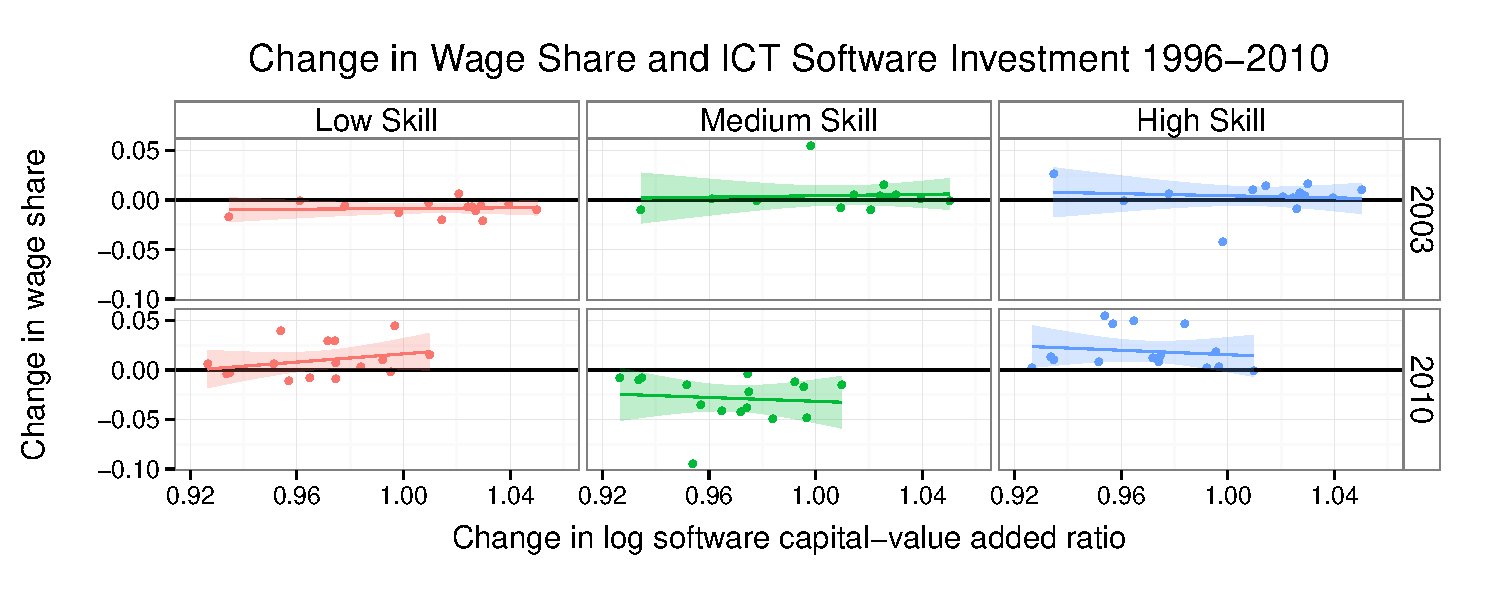
\includegraphics[width=0.8\textwidth]{../figure/wage_share_software_skill_split.pdf}
  \caption{Change in wage share against change in log ICT software capital ratio, by industry, Australia, 1996-2010. Fitted line comuted using LOESS regression and 95\% confidence interval.
    See note for Table~\ref{tbl:reg} for more details.
  }
  \label{fig:soft}
\end{figure}

\begin{figure}
  \centering
  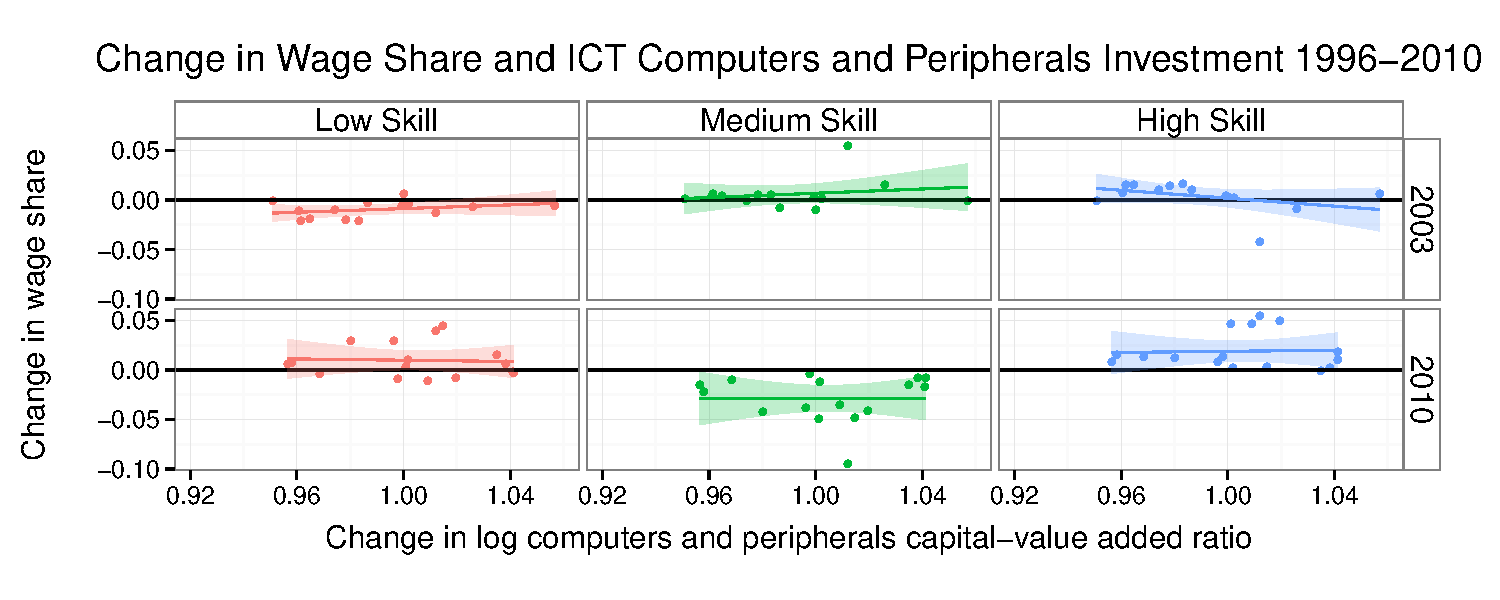
\includegraphics[width=0.8\textwidth]{../figure/wage_share_peripherals_skill_split.pdf}
  \caption{Change in wage share against change in log ICT computers and peripherals capital ratio, by industry, Australia, 1996-2010. Fitted line comuted using LOESS regression and 95\% confidence interval.
    See note for Table~\ref{tbl:reg} for more details.
  }
  \label{fig:periph}
\end{figure}

% Table created by stargazer v.4.0 by Marek Hlavac, Harvard University. E-mail: hlavac at fas.harvard.edu
% Date and time: Tue, Aug 27, 2013 - 22:20:32
% Requires LaTeX packages: dcolumn rotating 
\begin{sidewaystable}[!htbp] \centering 
  \caption{Wage Share Change Estimation Results: 1996-2010} 
  \label{tbl:reg} 
{\scriptsize
\begin{tabular}{@{}lD{.}{.}{-3} D{.}{.}{-3} D{.}{.}{-3} D{.}{.}{-3} D{.}{.}{-3} D{.}{.}{-3} D{.}{.}{-3} D{.}{.}{-3} D{.}{.}{-3} } 
\\[-1.8ex]\hline 
\hline \\[-1.8ex] 
 & \multicolumn{9}{c}{\textit{Dependent variable:}} \\ 
\cline{2-10} 
\\[-1.8ex] & \multicolumn{3}{c}{$\Delta SHARE^H$} & \multicolumn{3}{c}{$\Delta SHARE^M$} & \multicolumn{3}{c}{$\Delta SHARE^L$} \\ 
\\[-1.8ex] & \multicolumn{1}{c}{(1)} & \multicolumn{1}{c}{(2)} & \multicolumn{1}{c}{(3)} & \multicolumn{1}{c}{(4)} & \multicolumn{1}{c}{(5)} & \multicolumn{1}{c}{(6)} & \multicolumn{1}{c}{(7)} & \multicolumn{1}{c}{(8)} & \multicolumn{1}{c}{(9)}\\ 
\hline \\[-1.8ex] 
 $\Delta$log {\em equipment} & 0.931 &  &  &  &  &  &  &  &  \\ 
  & (0.699) &  &  &  &  &  &  &  &  \\ 
  & & & & & & & & & \\ 
 $\Delta$log {\em software} & -0.0001 &  &  & 0.454 &  &  & -1.444 &  &  \\ 
  & (1.625) &  &  & (1.369) &  &  & (1.303) &  &  \\ 
  & & & & & & & & & \\ 
 $\Delta$log {\em other capital} &  & 0.653 &  & -0.964^{*} & -0.883^{**} &  & 0.328 & 0.095 &  \\ 
  &  & (0.532) &  & (0.490) & (0.432) &  & (0.466) & (0.413) &  \\ 
  & & & & & & & & & \\ 
 $\Delta$log {\em value added} &  &  & -0.131 & 0.082 &  & -0.025 & -0.040 &  & -0.010 \\ 
  &  &  & (0.537) & (0.440) &  & (0.441) & (0.419) &  & (0.414) \\ 
  & & & & & & & & & \\ 
 Constant & 1.373 & 1.157 & 0.553 & -0.343 & -0.724 & -0.077 & 0.228 & 1.273 & 1.193 \\ 
  & (1.613) & (1.113) & (1.138) & (1.376) & (0.903) & (0.935) & (1.309) & (0.864) & (0.877) \\ 
  & & & & & & & & & \\ 
 Constant & -0.049 & -0.032 & -0.013 & 0.014 & 0.035 & 0.019 & -0.032 & -0.088 & -0.086 \\ 
  & (0.095) & (0.073) & (0.077) & (0.082) & (0.059) & (0.063) & (0.078) & (0.057) & (0.060) \\ 
  & & & & & & & & & \\ 
\hline \\[-1.8ex] 
Observations & \multicolumn{1}{c}{112} & \multicolumn{1}{c}{112} & \multicolumn{1}{c}{112} & \multicolumn{1}{c}{112} & \multicolumn{1}{c}{112} & \multicolumn{1}{c}{112} & \multicolumn{1}{c}{112} & \multicolumn{1}{c}{112} & \multicolumn{1}{c}{112} \\ 
R$^{2}$ & \multicolumn{1}{c}{0.023} & \multicolumn{1}{c}{0.017} & \multicolumn{1}{c}{0.004} & \multicolumn{1}{c}{0.038} & \multicolumn{1}{c}{0.037} & \multicolumn{1}{c}{0.0001} & \multicolumn{1}{c}{0.032} & \multicolumn{1}{c}{0.020} & \multicolumn{1}{c}{0.020} \\ 
Adjusted R$^{2}$ & \multicolumn{1}{c}{-0.005} & \multicolumn{1}{c}{-0.001} & \multicolumn{1}{c}{-0.014} & \multicolumn{1}{c}{0.002} & \multicolumn{1}{c}{0.019} & \multicolumn{1}{c}{-0.018} & \multicolumn{1}{c}{-0.005} & \multicolumn{1}{c}{0.003} & \multicolumn{1}{c}{0.002} \\ 
Residual Std. Error & \multicolumn{1}{c}{0.395 (108)} & \multicolumn{1}{c}{0.394 (109)} & \multicolumn{1}{c}{0.397 (109)} & \multicolumn{1}{c}{0.323 (107)} & \multicolumn{1}{c}{0.320 (109)} & \multicolumn{1}{c}{0.326 (109)} & \multicolumn{1}{c}{0.307 (107)} & \multicolumn{1}{c}{0.306 (109)} & \multicolumn{1}{c}{0.306 (109)} \\ 
F Statistic & \multicolumn{1}{c}{0.830 (3; 108)} & \multicolumn{1}{c}{0.957 (2; 109)} & \multicolumn{1}{c}{0.231 (2; 109)} & \multicolumn{1}{c}{1.065 (4; 107)} & \multicolumn{1}{c}{2.096 (2; 109)} & \multicolumn{1}{c}{0.004 (2; 109)} & \multicolumn{1}{c}{0.874 (4; 107)} & \multicolumn{1}{c}{1.139 (2; 109)} & \multicolumn{1}{c}{1.112 (2; 109)} \\ 
\hline 
\hline \\[-1.8ex] 
\textit{Note:}  & \multicolumn{9}{r}{$^{*}$p$<$0.1; $^{**}$p$<$0.05; $^{***}$p$<$0.01} \\ 
\normalsize 
\end{tabular}
}
{\em Wage shares computed for full-time workers, whose primary sources of income are wages and salaries, estimated for 16 industry groups. `High skill' workers include professionals and managers, `middle skill' workers include sales persons, clerical workers and para-professionals, and `low skill' workers include jobs with a high degree of manual activity, including laborers, transport workers and trades persons. To smooth out noise, all variables are estimated in seven-year differences. Survey data are composition adjusted by age bracket, sex and education level to be consistent with 2010 demographics. The variables {\em equipment} and {\em software} respectively refer to the capital stock of electronic and electrical equipment and computer software, at the end of each period. {\em other capital} refers to non-ICT capital, and {\em `value added'} is the value added for that industry group. Source: ABS (Survey of Income and Housing and National Accounts).}
\end{sidewaystable} 

These results should be interpreted with caution. Since there is no obvious natural experiment, and nor is there a clear instrument for ICT expenditure, this relationship should be interpreted simply as a correlation. Furthermore, it is unlikely that the level of ICT capital can be considered exogenous, since it is a substitute for endogenously-chosen middle-skilled labor. Nonetheless, the preceding analysis supports the more `nuanced' view that occupational tasks, rather than other human capital variables, are important determinants of the evolution of the wage distribution.

\section{Conclusions}

The evidence given above is only informal, although it is highly suggestive of a process of polarization in the Australian work force, consistent with patterns found in other labor markets. The results discussed so far also strongly suggest the simple SBTC story does not explain the evolution of the wage distribution in Australia. To wit, the notion of a `skill premium' is problematic in that, in this analysis, educational attainment appears to be a poor proxy of an individual's level of `skill.' Secondly, changes in the distribution of earnings as a result of technological change, appear to depend crucially on the nature of the job, rather than the level of skill it requires that workers possess.

% log-normality of income distribution: \cite{Willis2004}


%%% Local Variables: 
%%% mode: latex
%%% TeX-master: "paper"
%%% End: 
